\section{Method}
\label{sec:method}

\begin{figure*}[t]
\centering
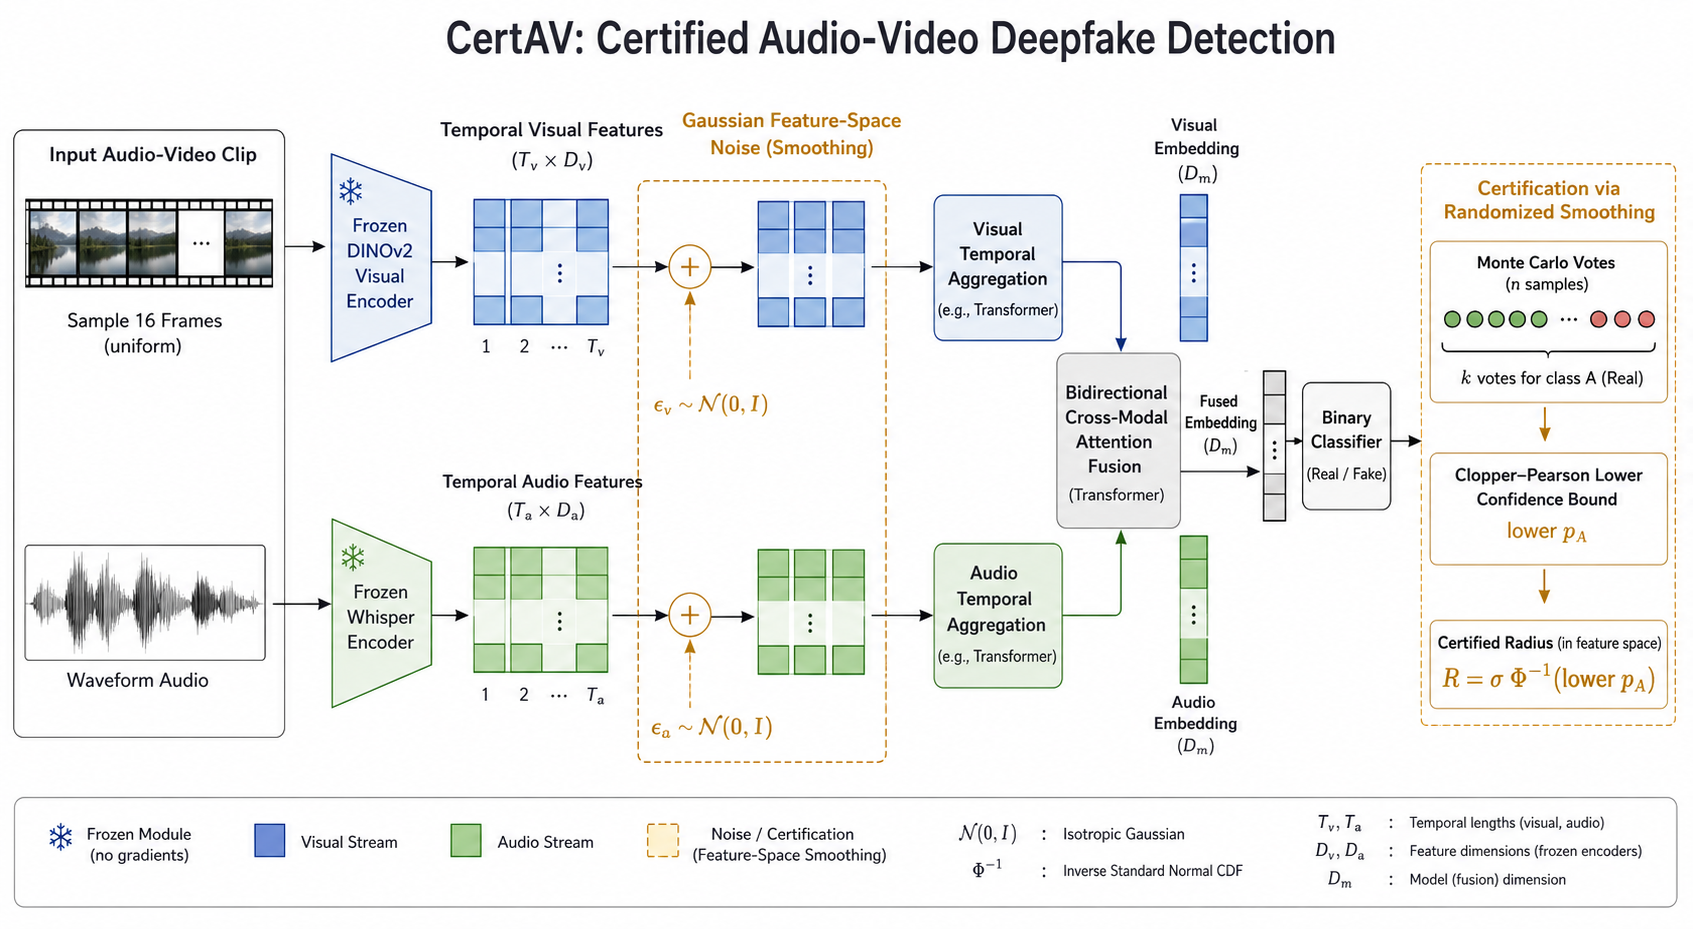
\includegraphics[width=0.95\textwidth]{figures/certav_architecture.png}
\caption{\textbf{CertAV pipeline.} Frozen DINOv2 and Whisper encoders produce temporal visual and audio features. A transformer aggregator and temporal pooling map each modality to a $256$-d sequence; a two-layer bidirectional cross-modal attention module fuses them; segment logits are averaged into a binary real/fake decision. Certification injects Gaussian (isotropic or PCA-aligned anisotropic) noise in the joint feature space and returns a prediction, an abstention flag, and an $\ell_2$ certified radius.}
\label{fig:arch}
\end{figure*}

\subsection{Feature extraction and detector}
\label{ssec:detector}

Given an audio-video clip $\x=(\x_v,\x_a)$, CertAV extracts frozen feature sequences $Z_v=E_v(\x_v)$ and $Z_a=E_a(\x_a)$. The visual encoder $E_v$ is a frozen DINOv2-Small ViT~\cite{oquab2024dinov2} applied to $16$ sampled frames, returning $384$-d frame embeddings. The audio encoder $E_a$ is the frozen Whisper-tiny encoder~\cite{radford2023whisper} over $16$\,kHz audio up to $10$\,s, returning $384$-d temporal embeddings. Features are cached in \texttt{float16} and used as the common input domain for training, attacks, and certification, which keeps certification tractable: the expensive encoders run once.

The detector $f_\theta$ has three stages. (1) \emph{Temporal aggregation}: each modality is projected $384\!\to\!256$; the visual branch adds learned positional embeddings and one transformer encoder layer ($8$ heads, $4\times$ feed-forward, dropout $0.1$) with adaptive pooling to $8$ segments, while the audio branch uses adaptive pooling and layer normalization. (2) \emph{Cross-modal consistency}: two bidirectional attention layers let visual tokens attend to audio and vice versa, with residual connections and a $512\!\to\!256$ fusion projection. (3) \emph{Classification}: a layer-normalized MLP ($256\!\to\!128\!\to\!1$, ReLU, dropout $0.3$) produces per-segment logits that are averaged into a single real/fake score.

\subsection{Threat model}
\label{ssec:threat}

Let $\z=(Z_v,Z_a)\in\RR^D$ with $D=768$ be the concatenated frozen representation. CertAV certifies robustness to a joint AV feature perturbation $\del=(\delta_v,\delta_a)$ with
\begin{equation}
\|\del\|_2 \le r .
\end{equation}
This threat model is narrower than raw waveform/pixel certification, but it is \emph{exact} for any adversary that operates on the representation the detector consumes, and it is the correct abstraction for the foundation-model era of forensics. Pixel/waveform certification of frozen billion-parameter encoders is computationally intractable and yields vanishingly small radii; meanwhile, adversaries in API-based or modular pipelines frequently target feature embeddings directly. Crucially, our geometric analysis (Sec.~\ref{sec:theory}) concerns the \emph{representational} geometry, which is independent of the input modality. To connect feature radii back to input space we further compose the certificate with an empirically estimated feature-to-input Lipschitz constant $L$: on FakeAVCeleb $L\!\approx\!50$, mapping the on-manifold certificate to an approximate input-space radius of $\approx\!0.12$ at $\approx\!90.7\%$ composed certified accuracy. We label this an empirical bridge, not a worst-case formal proof, and report it in Sec.~\ref{sec:exp}. Restricting $\del$ to one modality gives unimodal certificates (Sec.~\ref{sec:exp}); these can have larger numerical radii but protect a strictly smaller threat set.

\subsection{Isotropic randomized smoothing}
\label{ssec:iso}

We train with feature-space noise augmentation: $\tilde\z=\z+\eps$, $\eps\sim\mathcal{N}(0,\sigma^2 I)$, optimizing binary cross-entropy. The smoothed classifier is
\begin{equation}
g(\z)=\arg\max_{c\in\{0,1\}}\Pr_{\eps\sim\mathcal{N}(0,\sigma^2 I)}\!\left[f_\theta(\z+\eps)=c\right].
\label{eq:smoothed}
\end{equation}
Certification follows Cohen et al.~\cite{cohen2019certified}: $n_0=100$ Monte Carlo samples select the candidate class $A$; $n=1000$ samples estimate $p_A$; a one-sided Clopper-Pearson lower bound $\punder$ at significance $\alpha=0.001$ gives, if $\punder>0.5$, the certified radius
\begin{equation}
\Rcert=\sigma\,\Phi^{-1}(\punder),
\label{eq:cohen}
\end{equation}
and abstention otherwise. Certified accuracy at radius $r$ is the fraction of test clips that are correct, non-abstained, and satisfy $\Rcert\ge r$.

\subsection{Manifold-aware anisotropic smoothing}
\label{ssec:aniso}

Isotropic noise spends its budget equally in all $D$ directions. Sec.~\ref{sec:theory} shows that the detector is (approximately) invariant off the data manifold, so this is wasteful. We therefore smooth with $\eps\sim\mathcal{N}(0,\Sigma)$ where $\Sigma=U\,\mathrm{diag}(\lambda_1,\dots,\lambda_D)\,U^\top$ is diagonal in the PCA basis $U$ of the training features. Let $\Smanifold$ be the span of the top $d$ principal components ($90\%$ variance, $d\!\approx\!80$). We compare three budget-preserving strategies:
\begin{itemize}
\itemsep0.15em
\item \textbf{S1 (eigenvalue-proportional):} $\lambda_i \propto$ the $i$-th feature variance --- more noise where the data varies most.
\item \textbf{S2 (subspace projection):} noise is concentrated within $\Smanifold$ and suppressed off it.
\item \textbf{S3 (inverse-eigenvalue):} $\lambda_i \propto 1/(\text{variance})$ --- more noise in low-variance directions.
\end{itemize}
All three are normalized to the \emph{same} total budget as isotropic smoothing,
\begin{equation}
\mathrm{trace}(\Sigma)=\textstyle\sum_i \lambda_i = D\sigma^2,
\label{eq:budget}
\end{equation}
so any improvement comes from \emph{redistributing} noise, not from using more of it (verified in code: the raw per-direction variances are rescaled so their sum equals $D\sigma^2$). Because the certified region is now an ellipsoid rather than a ball, a single $\ell_2$ radius is no longer the natural summary; we report two complementary quantities.

\begin{definition}[On-manifold certified radius]
For anisotropic noise with covariance $\Sigma$ in the PCA basis,
$R_{\Smanifold}=\Phi^{-1}(\punder)\,\sqrt{\bar\lambda_{\Smanifold}}$, where $\bar\lambda_{\Smanifold}$ is the mean variance over the top-$d$ (on-manifold) directions. It measures the certified distance \emph{within} the subspace where the decision boundary lies.
\end{definition}

\begin{definition}[Worst-case $\ell_2$ radius]
$R_{\ell_2}=\Phi^{-1}(\punder)\,\sqrt{\lambda_{\min}(\Sigma)}$ is the radius of the largest sphere inscribed in the certified ellipsoid --- the guarantee against an adversary free to choose the \emph{worst} direction.
\end{definition}

\subsection{Robust conformal prediction}
\label{ssec:conformal}

CertAV abstains when $\punder\le 0.5$, leaving those samples without a guarantee. We add a distributional guarantee that covers \emph{every} sample. Using a held-out calibration set, split conformal prediction~\cite{romano2020classification,angelopoulos2023conformal} forms prediction sets $C_\alpha(\z)\subseteq\{\text{real},\text{fake}\}$ with marginal coverage $\Pr[y\in C_\alpha(\z)]\ge 1-\alpha$. We take the nonconformity score from the smoothed classifier's confidence and, following Gendler et al.~\cite{gendler2022adversarially}, form a \emph{robust} variant that inflates the calibrated threshold so that coverage is retained under any feature perturbation of radius $\le r$. For a forensic analyst, the set $\{\text{real},\text{fake}\}$ (uncertain but covered) is more actionable than ``no certificate available.''
